\documentclass{mynote}

\begin{document}
\title{(仮題)冒険者ちゃんとの日常 企画書}
\date{}
\maketitle

バトルありエロありの冒険者生活シミュレーション

タグ: 男主人公、おさわり、ファンタジー、日常/生活、いちゃラブ、異種姦、オナニー

意識しているタイトル: 妹せいかつ
\section{概要}

相棒の冒険者ちゃんと一緒にクエストを受けたりダンジョンを攻略して、冒険者として生活していくシミュレーションゲーム。
\subsection{コンセプト}
しっかり遊べるエロゲーをつくる

\section{システム}
\subsection{信頼度}
冒険をこなしたり、日々のコミュニケーションによって、相棒との信頼関係を築こう。

あなたへの信頼が大きくなれば、ムチャな「お願い」にも答えてくれるかも?

\subsection{性欲}
あなたと冒険者ちゃんどちらにもあるパラメータ。

普通に生活してるとかすかに溜まっていく。ハプニング、泥酔、生存本能が高まったりしたあとに大きく上昇する。

性欲が高まってえっちをしないと、冒険者ちゃんはひとりえっちをしだす。覗き見することも可能だが、本職シーフなので並の隠密性能ではバレるので、何かしらうまい手段を見つけるか、スパートかかって余裕が無くなった頃に覗くとよい。

えっちやテンションが下がるイベントによって減少する。

\subsection{気力}
日々頑張るために必要なもの。

何かしら行動するたびに減る。休んだりご飯を食べたりすると回復する。

\section{冒険}
ダンジョンを探索したり、冒険者ギルドの依頼をこなしたりしてお金を稼ごう。

依頼をこなしていくと、冒険者ランクを上げるための「昇格クエスト」が受けられる。

冒険者ランクが上がると、利用可能な街の設備が増えたり、商店でランクの高い冒険者向けの商品を売ってくれるようになる。

クエストやダンジョンで物資や金を集めて、街の工房や商店で強い装備を揃えて、またダンジョンに潜る。ローグライト?

\subsection{ダンジョン探索}
ダンジョンに入り、タンジョン内を探索して、敵と遭遇すれば倒して素材をGET、物資を見つけたら回収して、生きて脱出する。

死亡エンドをつくるかは決めていないが、「緊急脱出ボタン」とか、「アリアドネの糸」みたいなアイテムはほしい。

深いところには強いモンスターや強い冒険者の遺品、地下深くに建設された超高度文明の異物などがあり、そのへんの貴重なアイテムは自分でダンジョンに潜らないと手に入らない。

\subsection{クエスト}
冒険者ギルドでクエストを受ける。

金が稼げたり、昇格すると街の高機能な設備が使えるようになったりする。

ダンジョンは素材やアイテムが手に入るが、あれは各自がやりたくてやってるだけなので金や報酬はもらえない。

\section{世界観}
冒険者がいて、冒険者ギルドがあって、ダンジョンがあって、魔力みたいなファンタジー要素が多少はある世界。

\subsection{冒険者ちゃんちゃん}
冒険者登録をしてぼっちだったところ、偶然この子もぼっちだった。

あなた(プレイヤー)が戦士職で、冒険者ちゃんちゃんがシーフ職で相性が良かったのでパーティを組むことにした。

\subsection{街}
あなたと冒険者ちゃんちゃんが活動している街。

近所にそこそこ深いダンジョンがあり、王都へのアクセスもいいので結構栄えてる。

\subsection{ダンジョン}
遺跡や洞窟などの総称。昔の技術・文明の残骸、住み着いたモンスターの素材、冒険者の遺品などのお宝を求めて多くの人間が訪れる。

\subsection{冒険者ギルド}
モンスター討伐、物品の納品、護衛etc\dots 何でもやる「冒険者」を管理するギルド。ファンタジー版 フ◯キャストみたいな機関。

それなりに役に立つので各自治体から補助金が出てるところもある。

デカくてどこにでもあるので、冒険者証が身分証代わりになっている。申し込むだけならギルドに行って1時間くらいで済むので、成人したら取りあえず加入する人も多い。

\section{街の設備}
\subsection{冒険者ギルド}
クエスト受注、素材買い取り、研修、チュートリアル、ランク昇格ができる。

他にもできることが増えたら実装したい。

\subsection{宿屋}
泊まれる。体力、スタミナ、精神力的な、日々頑張るために必要なパラメータ(ここもあとで考える)

グレードがある。低グレードの宿屋は壁が薄いし寝具の室も悪く、パラメータの回復も悪い。壁が薄いのでえっちすると壁ドンされる。

\subsection{酒場}
酒を買ったり飲めたりするところ。

冒険者ちゃんを酔わせるのに使えるほか、他の客から耳寄り情報を聞けたりする。たちの悪い酔っぱらいが冒険者ちゃんに近づく演習がしたい。

\subsection{路地裏}
怖いところ。

犯罪者探しとか、猫探しとかに使いたい。

\subsection{商店}
クエスト用アイテム、雑貨、武器防具、etc\dots

「金を使って何らかのモノやサービスを購入できる施設」として扱いたい。

あ、ラブホほしいです。やっすい宿屋でえっちすると壁薄いから壁ドンされて中断。みたいな演出がほしい。あとシーツを過剰に汚して追加料金課されたりして。

ラブホは汚しても怒られないし壁ドンもされないっつーことで。

\section{どういう作りでいくか}
\subsection{次元}
2Dで行きます。マップを映すならドットがいい。

\subsection{戦闘ビュー}
とりあえず知ってるものを列挙する

\begin{enumerate}
  \item 見下ろし(不思議のダンジョン)
  \item FPS(世界樹)
  \item 横ビュー(Darkest Dungeon)
\end{enumerate}

\begin{figure}[h]
  \centering
  \fboxsep=0pt            %画像と枠線をくっつける.
  \fboxrule=1pt            %枠線の太さを1ptにする.
  \begin{minipage}{0.3\textwidth}
    \centering
    \fbox{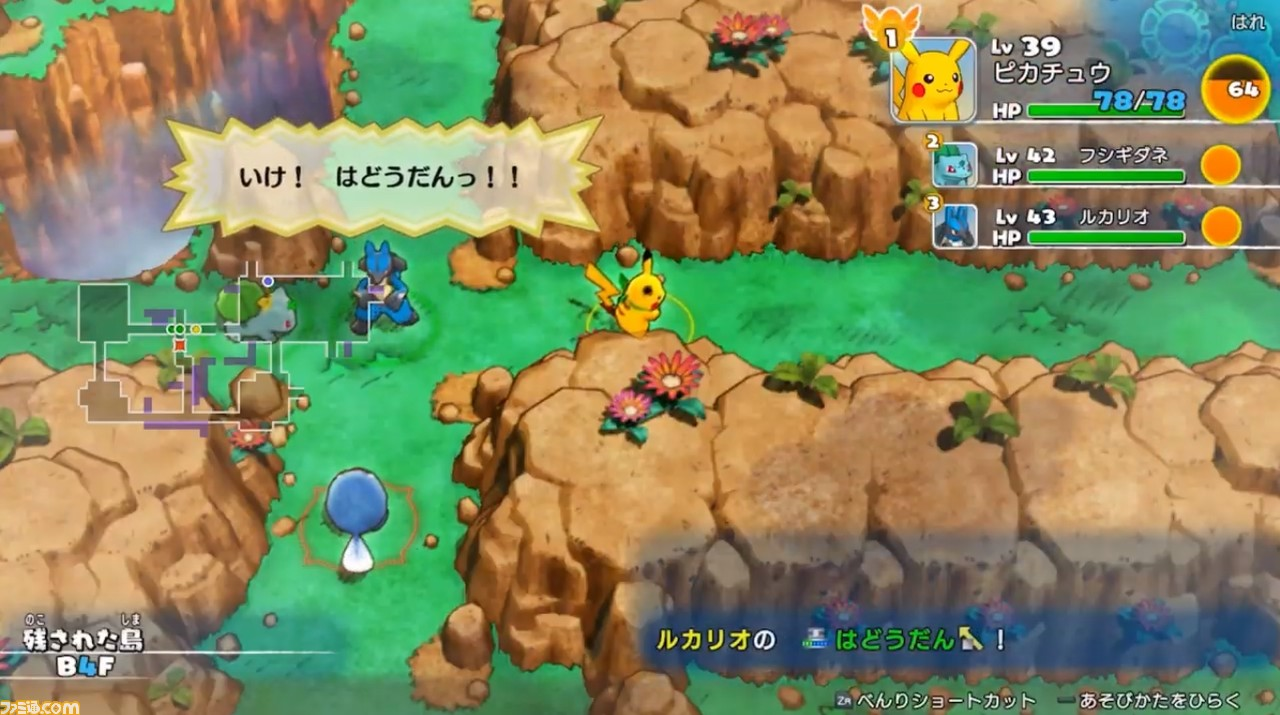
\includegraphics[keepaspectratio, clip, width=\textwidth]{Images/fushigi-no-dungeon.jpg}}
    \caption{見下ろし}
    \label{fig:fushigi-no-dungeon}
  \end{minipage}
  \hfill
  \begin{minipage}{0.3\textwidth}
    \centering
    \fbox{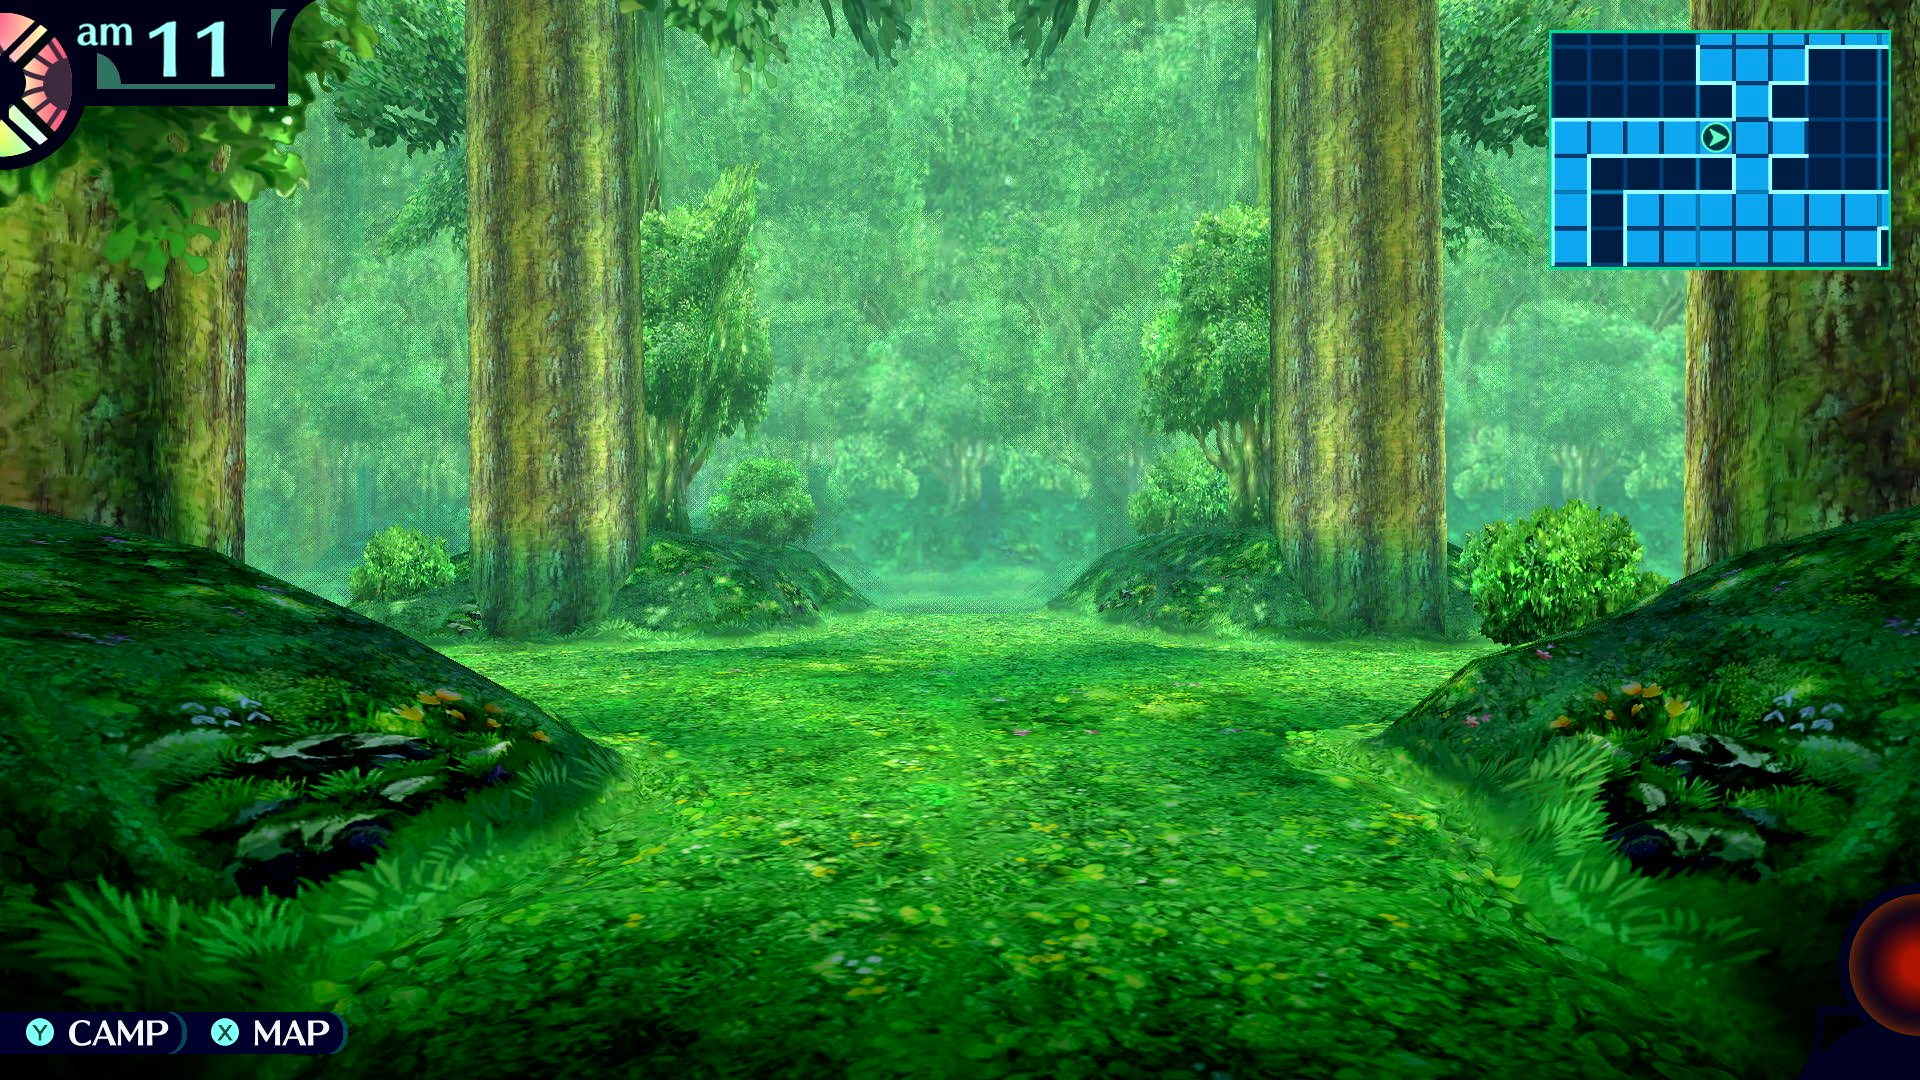
\includegraphics[keepaspectratio, clip, width=\textwidth]{Images/sekaiju-dungeon-view.jpg}}
    \caption{FPS}
    \label{fig:sekaiju-battle-view}
  \end{minipage}
  \hfill
  \begin{minipage}{0.3\textwidth}
    \centering
    \fbox{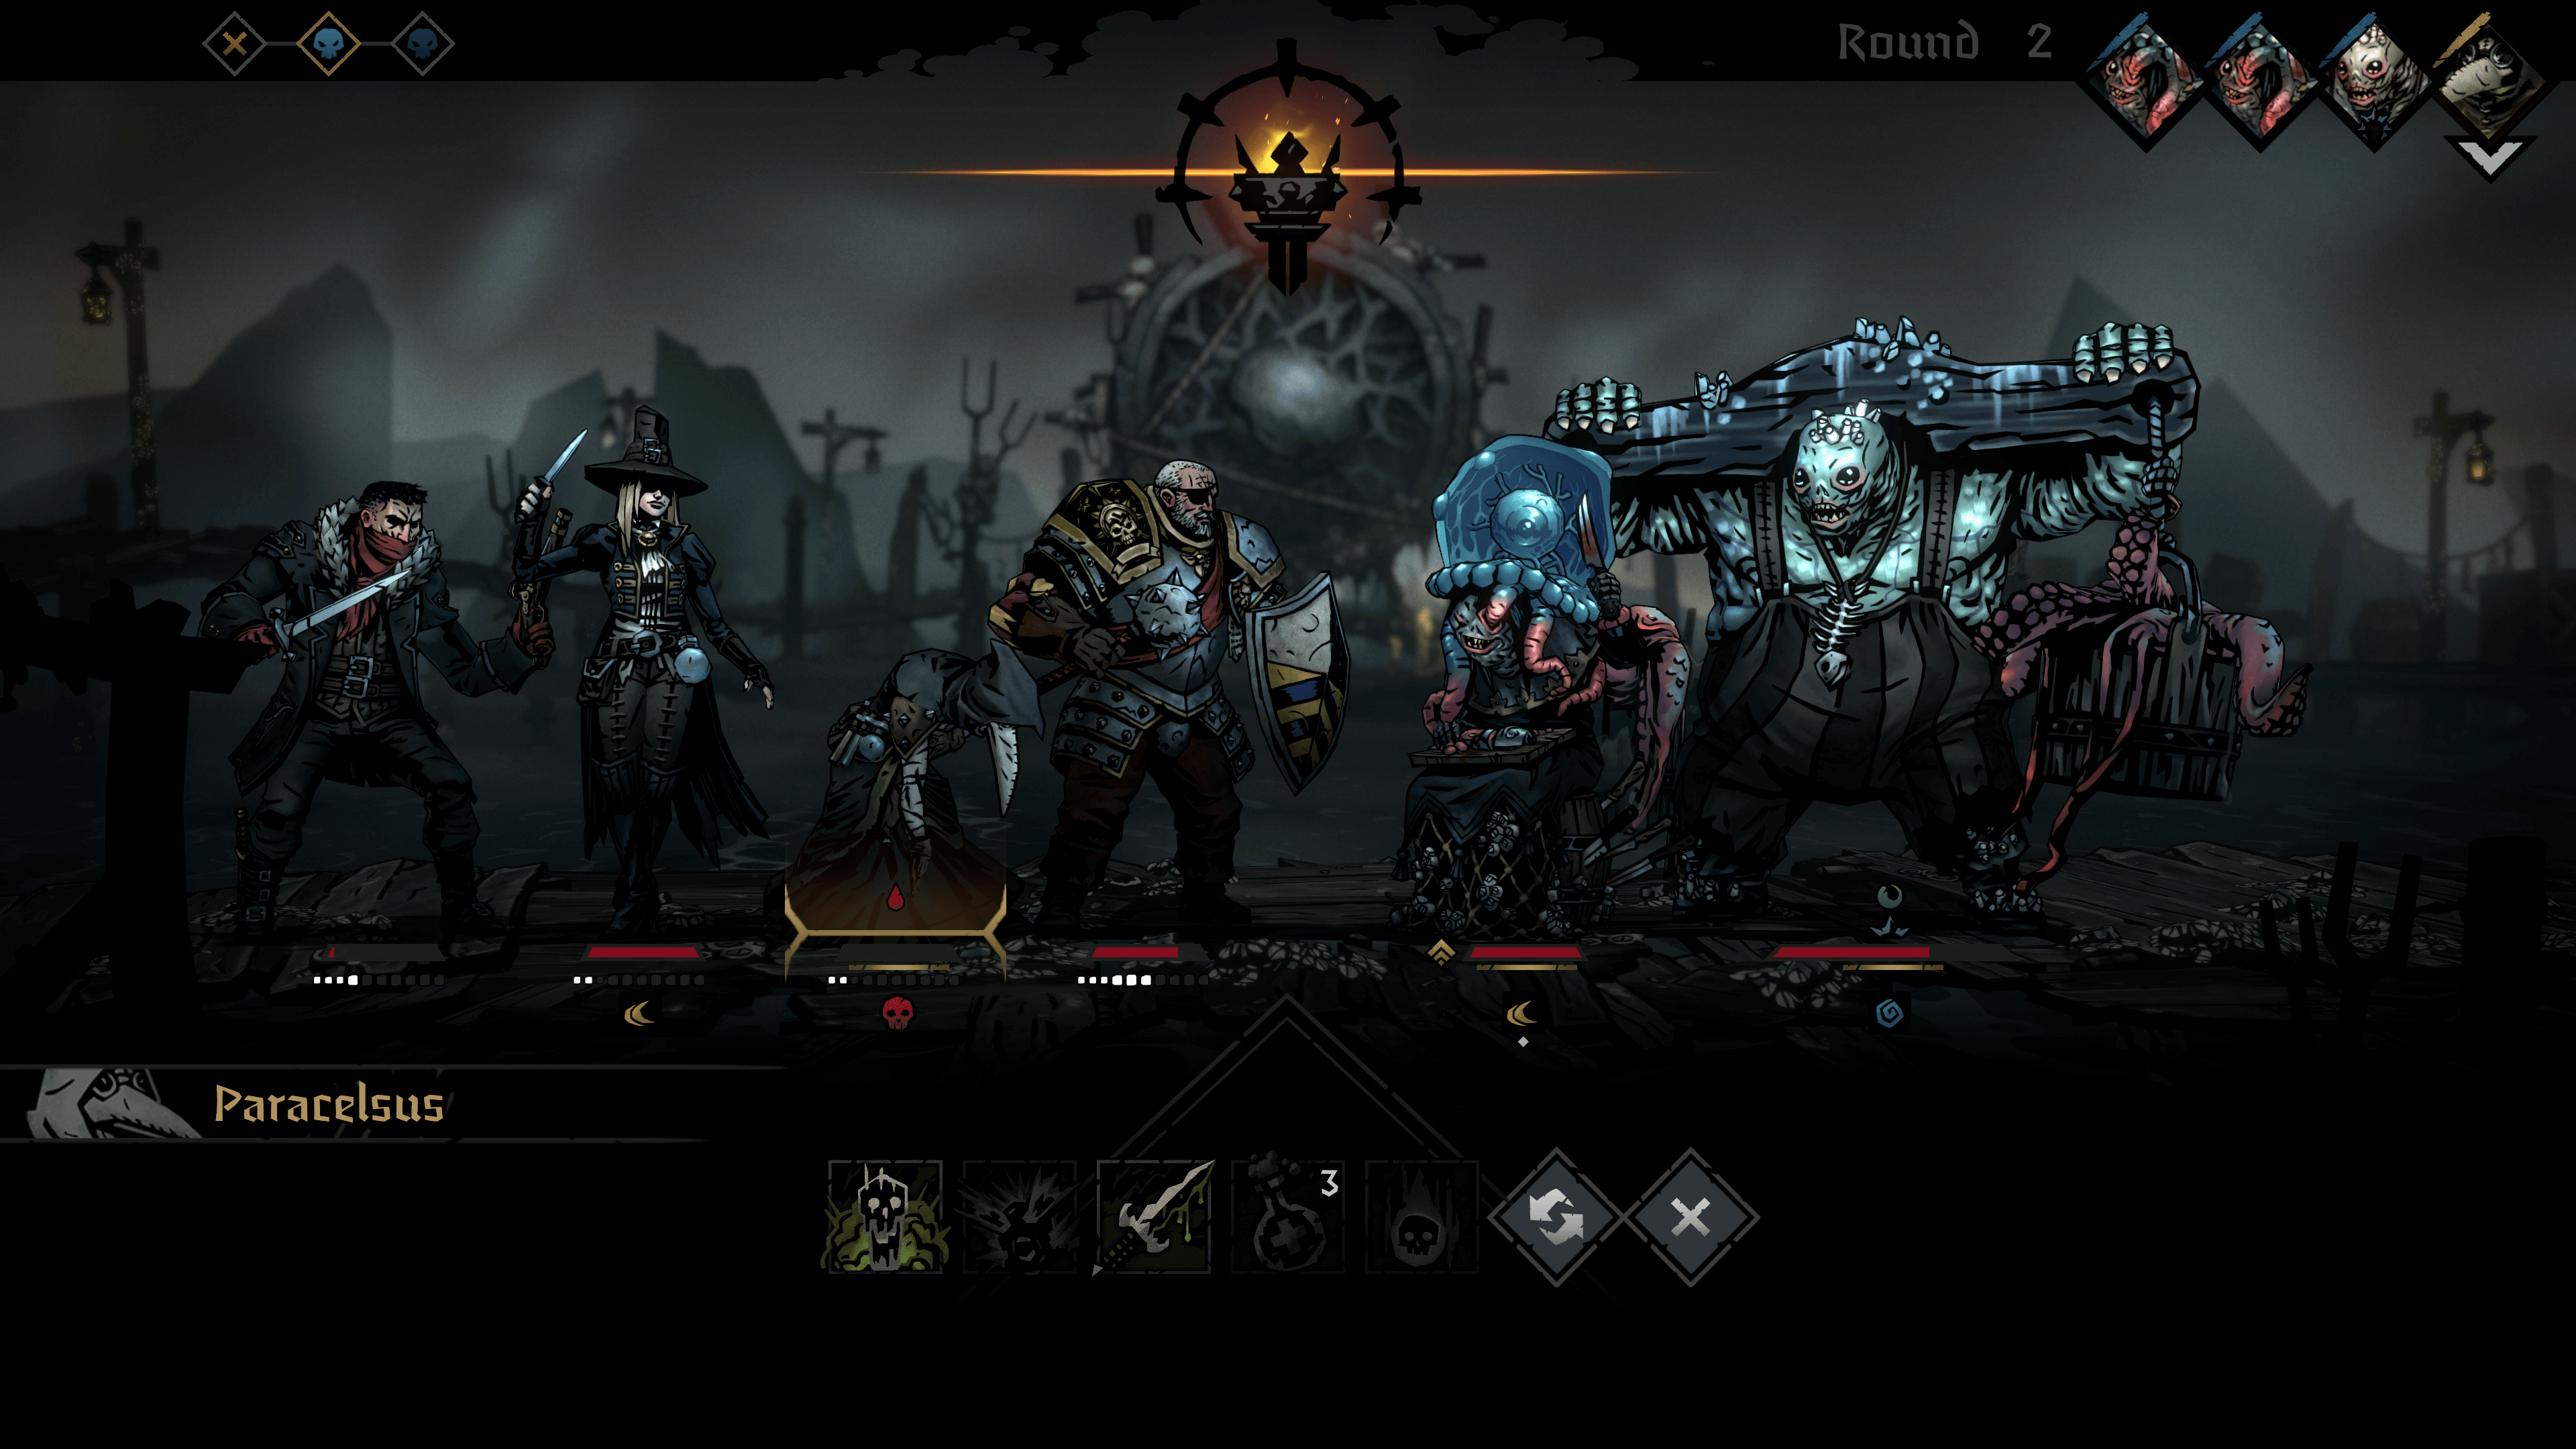
\includegraphics[keepaspectratio, clip, width=\textwidth]{Images/darkest-dungeon-battle-view.png}}
    \caption{横ビュー}
    \label{fig:darkest-dungeon-battle-view}
  \end{minipage}
\end{figure}

見下ろしが多分一番オーソドックス。今のところ見下ろしかなーと考えている。横ビューはアートワークの暴力が必要。無理。

戦闘ビューをダンジョン探索以外にも応用するのであれば、「特定の地点を目指す」とか、「話しかける」みたいなアクションを取りやすい構成がいいから、その点でも見下ろしがいいと思う。FPS?興味ないです。でも実はこっちのほうが工数減るとかあるのかな。

\subsection{「世界樹の迷宮」ライク or RPGツクールライク}

世界樹ライクの場合、探索やクエストのシステムに工夫が必要。世界観を感じる演出が難しいので、デザインに工夫が必要。

RPGツクールの場合、2次元のビューが常にあるので、2次元のシームレスな移動ができ、空間性を感じやすい。

2024.10.03時点では、世界樹ライクがいいかなと思う。システムの制約も少なそうなので拡張にしやすそう。とはいえわかりやすくフレームワークがあるのはツクールの方(偏見)だと思うので、世界樹ライクにするならそれなりの労力を想定する必要がある。

\section{技術選定}
今のところ知ってる技術だけで挙げると、
\begin{itemize}
  \item Unity
  \item UE5
  \item Godot
  \item RPGツクール MZ、MV
  \item Cocos2D
\end{itemize}

触り慣れてるのはUnity。触ったことがあるのもUnityのみ。

一人でも作りやすくて拡張しやすいミドルウェアがあれば勉強がてらやってみたい。

スクリプトは独自でもいいんだけど、できればC/C++を使うようなのがいい。C/C++好きだから。あと速いし。

\subsection{データの扱い}
Unity内で個々のデータをつくるのはだるそうだし、やめとけと\href{https://qiita.com/2dgames_jp/items/1730e7c4822091c3c320}{神}も言っていたので、それはやめようと思う。

excelもいいけど、jsonはvscodeだと扱いやすそうなので、今回は一旦jsonで扱うことにしようと思う。

\section{ToDo}
\subsection{ChatGPTからのFB(2024.10.03)}
\begin{itemize}
  \item ゲームプレイの方も充実させたシステムを考える
  \item 世界観の深堀り
  \item 技術選定の曖昧さ
  \item 個人開発で世界樹ライクは大変だぞ
  \item 冒険者ちゃんをちゃんと好きになれるように作り込め
  \item さっさと作って検証しろ
  \item 「いまどの行動をするか」を吟味できるようなゲームデザインにしろ
\end{itemize}

\end{document}
